\documentclass[11pt,english,a4paper,twoside,openright]{memoir}

%
% Our project name
%
\def\projectname{EPIC}
\def\pn{\textit{\projectname{}}}
\title{\pn{}}

%
% Contents = Table of Contents
%
\renewcommand{\contentsname}{Table of Contents}

%
% Packages
%
\usepackage{lmodern}
\usepackage{pifont}
\usepackage{memhfixc}
\usepackage[utf8]{inputenc}
\usepackage[T1]{fontenc}
\usepackage[english]{babel}
\usepackage[draft,english]{fixme}
\usepackage{graphicx}
\DisemulatePackage{setspace}
\usepackage{setspace}
\RequirePackage{lineno}
\usepackage{color}
\usepackage{calc}
\usepackage{soul}
\usepackage{textcomp}
\usepackage{pdfpages}
\usepackage{supertabular}
\usepackage{varioref}
\usepackage{listings}
\usepackage{tweaklist}
\usepackage{flafter}
\usepackage{multicol}
\usepackage{multirow}
\usepackage{rotating}
\usepackage{slashbox}
\usepackage{changepage}
\usepackage{longtable}
\usepackage{placeins}
\usepackage[pdftex,
            colorlinks=false,
            pdfduplex=DuplexFlipLongEdge,
            pdfborder={0 0 0},
            pdftitle={\projectname{}},
            pdfauthor={Group sw702a,
                7th semester Computer Science,
                AAU,
                Aalborg,
                Denmark},
            pdfsubject={Application Development},
            pdfkeywords={sw702a, LaTeX, .NET, C\#, MVC, ASP.NET, MVC 2, \projectname{}, Aalborg, aau},
            plainpages=false,
            bookmarksdepth=subsection
            ]{hyperref}

\usepackage{color}
\usepackage{colortbl}
\usepackage{amsmath}
\usepackage{expdlist}
\usepackage{fourier}

% Add hyphenation package and ignore font warnings (according to
% the official package documentation, they are all safe to ignore)
% This package is needed for breaking words in \texttt
%
\makeatletter
\let\my@@font@warning\@font@warning
\let\@font@warning\@font@info
\makeatother
%\usepackage[htt]{hyphenat}
\usepackage{hyphenat}
\makeatletter
\let\@font@warning\my@@font@warning
\makeatother



%
% Make a newline after paragraphs
%
\makeatletter
\renewcommand\paragraph{
   \@startsection{paragraph}{4}{0mm}
      {-\baselineskip}
      {.5\baselineskip}
      {\normalfont\normalsize\bfseries}}
\makeatother

%
% Make quotation environments italic
%
\makeatletter
\g@addto@macro{\quote}{\itshape}
\g@addto@macro{\quotation}{\itshape}
\makeatother
%
% FiXME package is using the margin as note, and the
% fixme text is appended to the footnote. The exact
% position of the fixme is marked with a indexy
%
\fxsetup{layout={marginclue,footnote,index},innerlayout=}

%
% New burl command... this is not that pretty
%
\newcommand{\burl}[1] {
	\href{#1}{\texttt{#1}}
}
\newcommand{\burlalt}[2] {
	\href{#1}{\texttt{#2}}
}

%
% Define a new column type
% Tabularx does not support a centered X column,
% so we will create our own
%
\newcolumntype{L}[1]{>{\raggedright\arraybackslash}p{#1}}

%
% Set line spacing
%
\setstretch{1.1}

%
% Set line number margin
%
\setlength{\linenumbersep}{1.5cm}

%
% Set no paragraph indent
%
\setlength{\parindent}{0pt}

%
% Redefine the indent command to make a horizontal space
%
\renewcommand{\indent}{\hspace{0.5cm}}

%
% Set itemize/enumeration/descripthook seperation (this is a small hack using tweaklist package :))
%
\renewcommand{\itemhook}{
	\setlength{\itemsep}{0pt}
}
\renewcommand{\descripthook}{
	\setlength{\itemsep}{0pt}
}

%  
% Enable subfigures in memoir
%
\newsubfloat{figure}
\newsubfloat{table}

%
% Margins
%
\setlrmarginsandblock{3.5cm}{*}{0.75} % Right and left
\setulmarginsandblock{3cm}{*}{1.2}    % Top and bottom

%
% Headings
% - Change normal headers and footers
%
\makeoddhead{headings}{}{}{\small\rightmark}
\makeevenhead{headings}{\small\leftmark}{}{}

\makeoddfoot{headings}{}{}{\small\thepage}
\makeevenfoot{headings}{\small\thepage}{}{}

\makeheadrule{headings}{\textwidth}{\normalrulethickness}
\makefootrule{headings}{\textwidth}{\normalrulethickness}{\footruleskip}

%
% Force LaTeX to not fill the page with extra vertical space
%
\raggedbottom

%
% Section titles
%
\settocdepth{subsection}
\setsecnumdepth{subsubsection}
\maxsecnumdepth{subsubsection}

%
% New chapter style
%
\definecolor{chapterbg}{rgb}{.45,.45,.45}
\makeatletter
\newlength\dlf@normtxtw
\setlength\dlf@normtxtw{\textwidth}
\def\myhelvetfont{\def\sfdefault{mdput}}
\newsavebox{\feline@chapter}
\newcommand\feline@chapter@marker[1][4cm]{%
\sbox\feline@chapter{%
\resizebox{!}{#1}{\fboxsep=1pt%
\colorbox{chapterbg}{\color{white}\bfseries\sffamily\thechapter}%
}}%
\rotatebox{90}{%
\resizebox{%
\heightof{\usebox{\feline@chapter}}+\depthof{\usebox{\feline@chapter}}}%
{!}{\scshape\so\@chapapp}}\quad%
\raisebox{\depthof{\usebox{\feline@chapter}}}{\usebox{\feline@chapter}}%
}
\newcommand\feline@chm[1][4cm]{%
\sbox\feline@chapter{\feline@chapter@marker[#1]}%
\makebox[0pt][l]{% aka \rlap
\makebox[1cm][r]{\usebox\feline@chapter}%
}}
\makechapterstyle{daleif1}{
\renewcommand\chapnamefont{\normalfont\Large\scshape\raggedleft\so}
\renewcommand\chaptitlefont{\normalfont\huge\bfseries\scshape\color{chapterbg}}
\renewcommand\chapternamenum{}
\renewcommand\printchaptername{}
\renewcommand\printchapternum{\null\hfill\feline@chm[2.5cm]\par}
\renewcommand\afterchapternum{\par\vskip\midchapskip}
\renewcommand\printchaptertitle[1]{\chaptitlefont\raggedleft ##1\par}
}
%
% Apply the chapter style
%
\makeatother
\chapterstyle{daleif1}

%
% Figure Captions
%
\captionnamefont{\bfseries\sffamily\small}
\captiontitlefont{\small}
\changecaptionwidth
\captionwidth{.8\textwidth}
\precaption{\vspace{\baselineskip}}


%
% Define colors used in source code boxes
%
\definecolor{red}{rgb}{1,0,0}
\definecolor{green}{rgb}{0,1,0}
\definecolor{yellow}{rgb}{1,1,0}
\definecolor{blue}{rgb}{0,0,1}
\definecolor{darkblue}{rgb}{0,0,0.5}
\definecolor{prggreen}{rgb}{0.18,0.55,0.34}
\definecolor{prgviolet}{rgb}{0.63,0.13,0.94}
\definecolor{prgred}{rgb}{0.65,0.16,0.16}
\definecolor{prgpink}{rgb}{1,0,1}
\definecolor{srcbg}{rgb}{.97,.97,.97}

%
% Source code boxes
%

\lstnewenvironment{source}[2][]{
    \def\lstlistingname{Source Code}
    \lstset{
    	aboveskip=0.5cm,
    	belowskip=0.5cm,
        linewidth=0.95\textwidth,
        xleftmargin=0.05\textwidth,
        basicstyle=\ttfamily\selectfont\small,
        extendedchars=true,
        columns=flexible,
        escapechar=\$,
        frame=lines,
        numbers=left,
        numberstyle=\tiny,
        numbersep=10pt,
        breaklines,
        tabsize=3,
        breakatwhitespace=true,
        showspaces=false,
        showstringspaces=false,
        language=Java,
        prebreak=\Pisymbol{psy}{191},
        emph={[1]root,base,public,private,protected,interface,abstract,class,throws,new,throwable},
        emphstyle={[1]\color{prgred}\bfseries},
        keywordstyle={[1]\bfseries},
        emph={[2]while,for,do,return,goto,if,else,switch,break,default,case},
        emphstyle={[2]\color{prggreen}},
        keywordstyle={[2]\bfseries},
        emph={[3]volatile,long,int,char,string,boolean,unsigned,void,external,double,byte,float},
        emphstyle={[3]\color{prggreen}\bfseries},
        keywordstyle={[3]\bfseries},
        morecomment=[l][\color{blue}]{//},
        morecomment=[s][\color{blue}]{/*}{*/},
        morecomment=[s][\color{prgpink}]{"}{"},
        captionpos=b,
        caption={#1},
        label={#2}
    }
}{}

\lstnewenvironment{pseudo}[2][]{
    \def\lstlistingname{Pseudo Code}
    \lstset{
    	aboveskip=0.5cm,
    	belowskip=0.5cm,
        linewidth=0.95\textwidth,
        xleftmargin=0.05\textwidth,
        basicstyle=\ttfamily\selectfont\small,
        extendedchars=true,
        columns=flexible,
        escapechar=\$,
        frame=lines,
        numbers=left,
        numberstyle=\tiny,
        numbersep=10pt,
        breaklines,
        tabsize=3,
        breakatwhitespace=true,
        showspaces=false,
        showstringspaces=false,
        language=C,
        prebreak=\Pisymbol{psy}{191},
        captionpos=b,
        caption={#1},
        label={#2}
    }
}{}

%
% Make a small indent in tables
%
\setlength{\tabcolsep}{10pt}

%
% Fix the page layout
%
\checkandfixthelayout[nearest]



%
% Old chapter style
%
\begin{comment}
\makechapterstyle{coolish}{
    \newif\ifchapternonum
    \renewcommand\printchaptername{}
    \renewcommand\printchapternum{}
    \renewcommand\printchapternonum{\chapternonumtrue}

    \renewcommand\printchaptertitle[1]{
        \reset@font
		\parindent \z@ 
		\vspace*{10\p@}
		\hbox{
		    \vbox{
                \hsize=2cm
		        \begin{tabular}{c}
				    \ifchapternonum
		                \scshape \strut \vphantom{\@chapapp{}} \hphantom{\@chapapp{}} \\
				    \else
				        \scshape \strut \@chapapp{} \\
				    \fi
                    \fbox{
                        \vrule depth 10em width 0pt
                        \vrule height 0pt depth 0pt width 1ex
                                      
                        \ifchapternonum
                              {\LARGE \bfseries \strut \hphantom{\thechapter}}
                        \else
                              {\LARGE \bfseries \strut \thechapter}
                        \fi
                        \vrule height 0pt depth 0pt width 1ex
                    }
                \end{tabular}
            }
            \vbox{
                \advance\hsize by -2cm
                \hrule\par
                \vskip 6pt
                \hspace{1em}
                \Huge \bfseries ##1
            }
        }
        \vskip 60\p@
    }
}
\end{comment}

%
% force breaks at right margin, if the text is too long
%
\sloppy
\begin{document}

% 
% Include front page pdf file
% 
%\includepdf{forside.pdf}

%
% Make a new empty page   
%
%\newpage
% Blank page after frontpage
%\mbox{}
%\thispagestyle{empty} 
%\newpage

% 
% Use roman numbers on the start of the report   
%
\pagenumbering{Roman}

% 
% Files for writing preface
%
\input{preface/titlepage}

\chapter*{Preface}
\chapter*{Preface}
This report is written in the fourth semester of the software engineering study at Aalborg University in the spring 2011.
\\
\\
The goal of this project is to acquire knowledge about fundamental principles of programming languages and techniques for description and translation of languages in general. Also a goal is to get a basic knowledge of central computer science and software technical subjects with a focus on language processing theories and techniques.\\
  We are going to achieve these goal by designing and implementing a small language for controlling a multi agent system in the form of a wargame. We are going to use Visual Studio and C\#, because we have used these tools in earlier semesters and are used to the C\# syntax.
	\\
	\\
	The report is written i \LaTeX, and we have used Google Docs and TortoiseSVN for revision control.
	\\

Source code examples in the report is represented as follows:
\begin{source}{This is a sorce code example}{}
if (spelling.ToLower().Equals(spellings[i]))
	{
		this.kind = i;
		break;
	}
\end{source}

% 
% Create table of contents
%
\newpage{}
%\changepage{2.5cm}{}{}{}{}{}{}{-2.5cm}{}% fix table of contents to fit 2 pages
\tableofcontents*
%\changepage{-2.5cm}{}{}{}{}{}{}{2.5cm}{}% fix table of contents to fit 2 pages

%
% Use temporary line numbers on all pages
%
%\setpagewiselinenumbers
%\linenumbers

%
% Main Contents of report, add chapters here
%

%
% Use arabic numbers in the rest of the report (is in introduction/intro.tex)
%
\chapter{Introduction}
\label{chap:intro}
\pagenumbering{arabic}
A basic compiler can be broken down to three simplet steps which are illustrated in \ref{fig:compiler}.

\begin{figure}[H]
\begin{center}
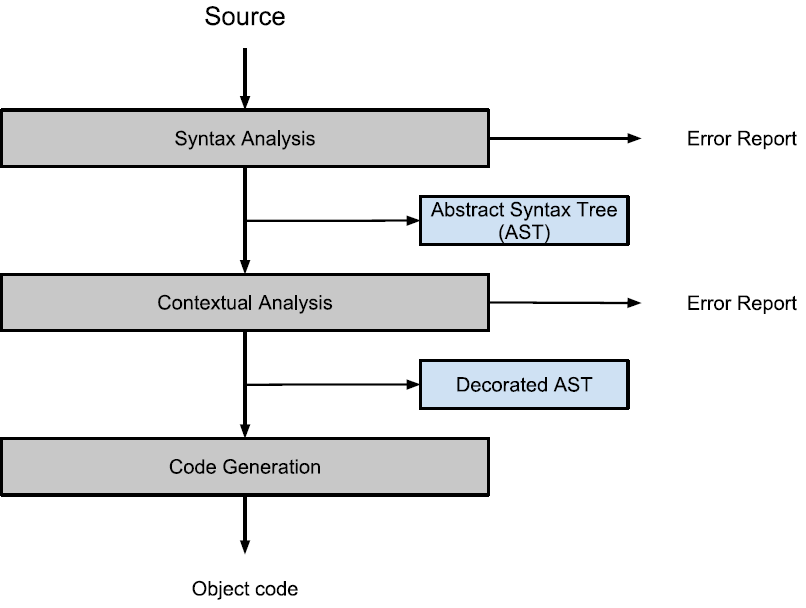
\includegraphics[scale=0.7]{Images/compiler_drawing.png}
\label{fig:compiler}
\caption{Illustration of the compiler components.}
\end{center}
\end{figure}
\newpage{}
%\input{introduction/readingguide}


\chapter{Analysis}
\label{chap:analysis}
A basic compiler can be broken down to three simplet steps which are illustrated in \ref{fig:compiler}.

\begin{figure}[H]
\begin{center}
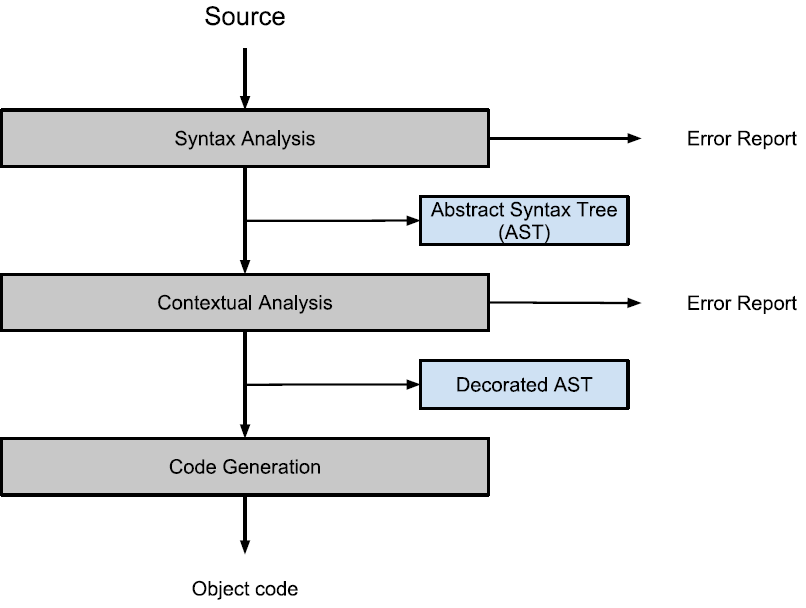
\includegraphics[scale=0.7]{Images/compiler_drawing.png}
\label{fig:compiler}
\caption{Illustration of the compiler components.}
\end{center}
\end{figure}
\newpage{}
\input{analysis/systemdefinition}
\input{analysis/eventtable}
\input{analysis/actors}
\input{analysis/usecases}
\input{analysis/functions}

\chapter{Design}
\label{chap:Design}


\chapter{Development}
\label{chap:development}
%A basic compiler can be broken down to three simplet steps which are illustrated in \ref{fig:compiler}.

\begin{figure}[H]
\begin{center}
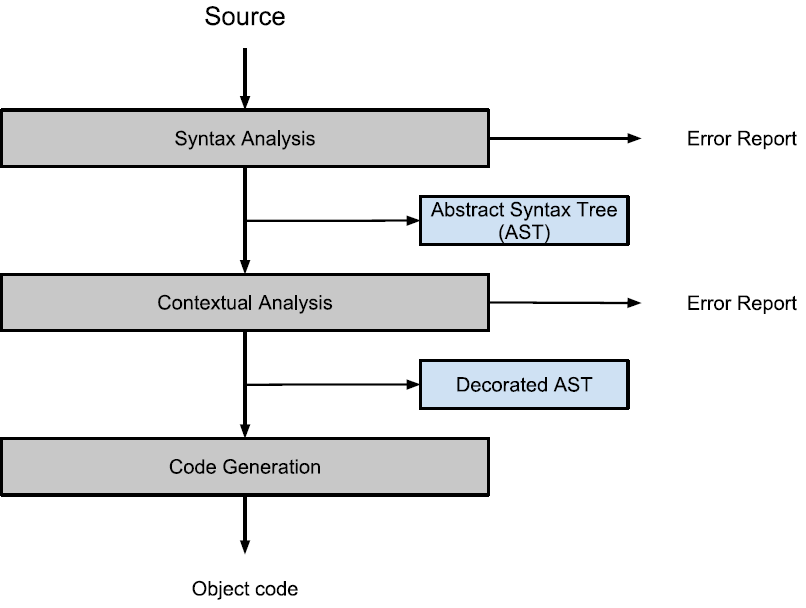
\includegraphics[scale=0.7]{Images/compiler_drawing.png}
\label{fig:compiler}
\caption{Illustration of the compiler components.}
\end{center}
\end{figure}
\newpage{}
%\input{developsubcomponent/initialsetup}
%\input{developsubcomponent/developmentapproach}
%\input{developsubcomponent/databaseaccesslayer}
%\input{developsubcomponent/calendar}
%\input{developsubcomponent/componentannouncer}

% Chapter: Integration
\chapter{Testing}
%A basic compiler can be broken down to three simplet steps which are illustrated in \ref{fig:compiler}.

\begin{figure}[H]
\begin{center}
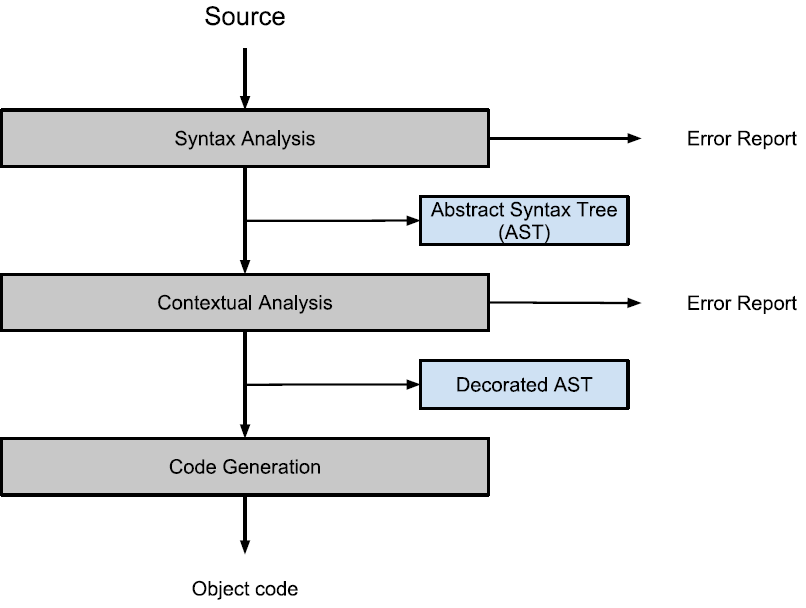
\includegraphics[scale=0.7]{Images/compiler_drawing.png}
\label{fig:compiler}
\caption{Illustration of the compiler components.}
\end{center}
\end{figure}
\newpage{}
%\input{testing/component}
%\input{testing/integration}
%\input{testing/system}

% Chapter: Reflection
\chapter{Reflection}
%A basic compiler can be broken down to three simplet steps which are illustrated in \ref{fig:compiler}.

\begin{figure}[H]
\begin{center}
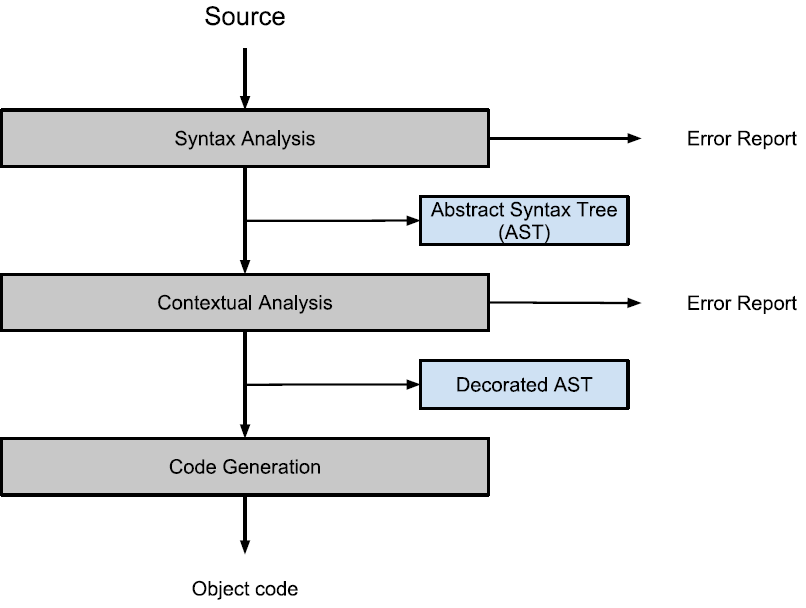
\includegraphics[scale=0.7]{Images/compiler_drawing.png}
\label{fig:compiler}
\caption{Illustration of the compiler components.}
\end{center}
\end{figure}
\newpage{}
%\input{reflection/developmentapproach}
%\input{reflection/components}
%\input{reflection/collaboration}

% Chapter: Recapitulation
\chapter{Recapitulation}
%A basic compiler can be broken down to three simplet steps which are illustrated in \ref{fig:compiler}.

\begin{figure}[H]
\begin{center}
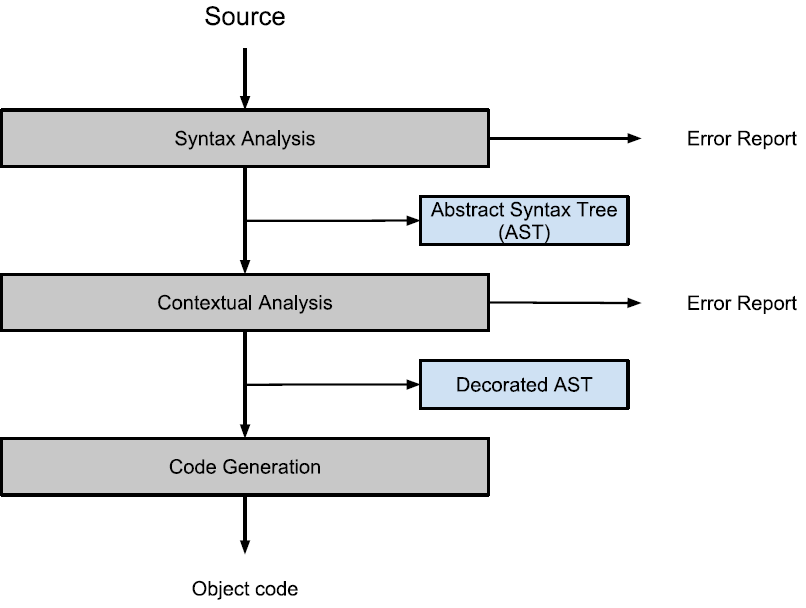
\includegraphics[scale=0.7]{Images/compiler_drawing.png}
\label{fig:compiler}
\caption{Illustration of the compiler components.}
\end{center}
\end{figure}
\newpage{}
%\chapter{Conclusion}
%\input{recapitulation/futurework}

\label{theend}
%
% Bibliography
%
%\bibliographystyle{alpha}
%\bibliography{references}
\label{bib}
%
% Creates an appendix 
%
\appendix
% Add appendix to toc
\addappheadtotoc
% Only add the chapters, and not sections, subsections etc.
\settocdepth{chapter}
%\input{appendix/contract}
%\input{appendix/userstories}
%\input{appendix/eventbehavior}
%\input{appendix/guimockups}
%\input{appendix/testscripts}
%\input{appendix/redmineguides}
%\input{appendix/unittestdescription}
%\input{appendix/resume}

\label{pagecount}
%
% A page used to attach the CD-ROM
%
\cleardoublepage
\thispagestyle{empty}
\vspace*{4cm}
\label{cd}
{\centering This page is left blank for the purpose of containing the attached CD-ROM.}

%
% FixME's chapter.. Should be commented when finished :)
%
\newpage
\chapter{FIXME's}
\listoffixmes

\end{document}
